\section{Auswertung} \label{sec:auswertung}

Im Folgenden sollen die Grenzspannung für verschiedene Wellenlängen bestimmt werden,
um daraus auf $\frac{h}{e}$ und Austrittsarbeit $A_\text{K}$ zu schließen.
Außerdem wird am Beispiel des Photostroms gelben Lichts
auf Charakteristika der Spannungs-Strom-Kurve wie Sättigungseffekte eingeganen.

\begin{table}
  \centering
  \caption{Messreihe für gelbes Licht (hier wurde ein größerer Spannungsbereich gemessen; siehe \autoref{sec:auswertung:gelb_full}).}
  \label{tab:werte_gelb}
  \begin{tabular}{S S}
  \toprule
  $U_g \mathbin{/} \si{\volt}$ &
  $I \mathbin{/} \si{\nano\ampere}$ \\
  \midrule
  \expandableinput{build/table_gelb.tex}
  \bottomrule
  \end{tabular}
\end{table}

\begin{table}
  \centering
  \caption{Messreihe für grünes Licht.}
  \label{tab:werte_gruen}
  \begin{tabular}{S S}
  \toprule
  $U_g \mathbin{/} \si{\volt}$ &
  $I \mathbin{/} \si{\nano\ampere}$ \\
  \midrule
  \expandableinput{build/table_gruen.tex}
  \bottomrule
  \end{tabular}
\end{table}

\begin{table}
  \centering
  \caption{Messreihe für violettes Licht.}
  \label{tab:werte_violett}
  \begin{tabular}{S S}
  \toprule
  $U_g \mathbin{/} \si{\volt}$ &
  $I \mathbin{/} \si{\nano\ampere}$ \\
  \midrule
  \expandableinput{build/table_violett.tex}
  \bottomrule
  \end{tabular}
\end{table}

\begin{table}
  \centering
  \caption{Messreihe für ultraviolettes Licht.}
  \label{tab:werte_ultraviolett}
  \begin{tabular}{S S}
  \toprule
  $U_g \mathbin{/} \si{\volt}$ &
  $I \mathbin{/} \si{\nano\ampere}$ \\
  \midrule
  \expandableinput{build/table_ultraviolett.tex}
  \bottomrule
  \end{tabular}
\end{table}

% \clearpage
\subsection{Bestimmung der Grenzspannung für verschiedene Wellenlängen}

Aus dem in \autoref{eqn:sqrt_I_gesetz} beschriebenen Zusammenhang folgt, dass $\sqrt{I_\text{Ph}} \propto U$ ist.
Um die Grenzspannung über eine Regressionsgerade zu bestimmen,
wird daher $\sqrt{I_\text{Ph}}$ gegen $U$ aufgetragen
und der Achsenabschnitt $U_g$ der Ausgleichgerade
\begin{equation*}
  \sqrt{I} = aU + b
\end{equation*}
gemäß
\begin{equation*}
    U_g = - \frac{a}{b}
\end{equation*}
berechnet.
Die nachstehenden Plots visualisieren dieses Vorgehen für die verschiedenen Wellenlängen.
Dargestellt ist jedoch nur der zu betrachtende lineare Abschnitt.
Die vollständigen Daten finden sich in den jeweiligen Tabellen
(\ref{tab:werte_gelb}, \ref{tab:werte_gruen}, \ref{tab:werte_violett}, \ref{tab:werte_ultraviolett}).

\begin{figure}[H]
    \centering
    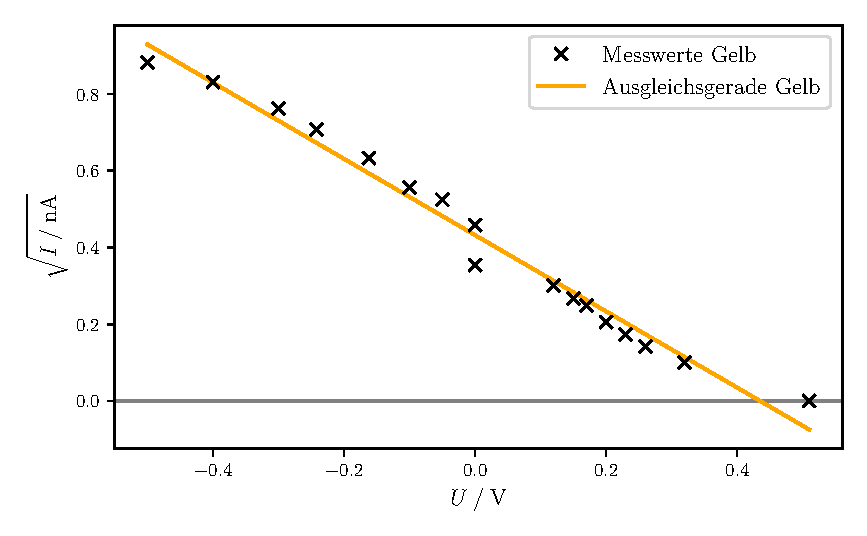
\includegraphics[width=0.8\textwidth]{build/plot_sqrt_gelb.pdf}
    \caption{Die Wurzel des Photostroms und ihre Ausgleichgerade für gelbes Licht, aufgetragen gegen die Spannung.}
    \label{fig:plot_sqrt_gelb}
\end{figure}

\begin{figure}[H]
    \centering
    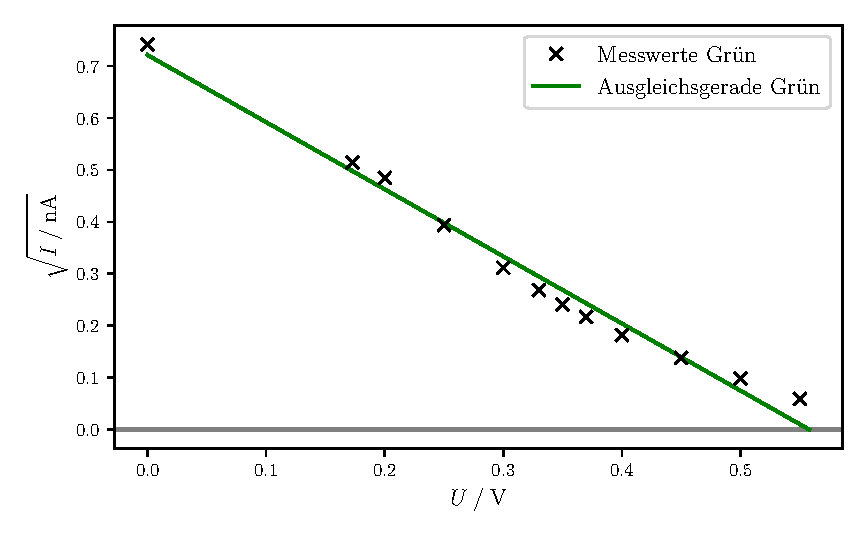
\includegraphics[width=0.8\textwidth]{build/plot_sqrt_gruen.pdf}
    \caption{Die Wurzel des Photostroms und ihre Ausgleichgerade für grünes Licht, aufgetragen gegen die Spannung.}
    \label{fig:plot_sqrt_gruen}
\end{figure}

\begin{figure}[H]
    \centering
    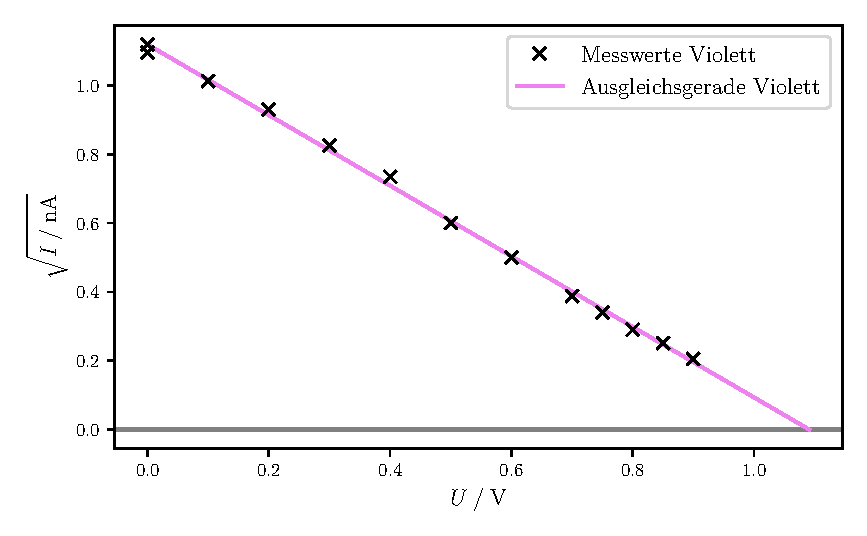
\includegraphics[width=0.8\textwidth]{build/plot_sqrt_violett.pdf}
    \caption{Die Wurzel des Photostroms und ihre Ausgleichgerade für violettes Licht, aufgetragen gegen die Spannung.}
    \label{fig:plot_sqrt_violett}
\end{figure}

\begin{figure}[H]
    \centering
    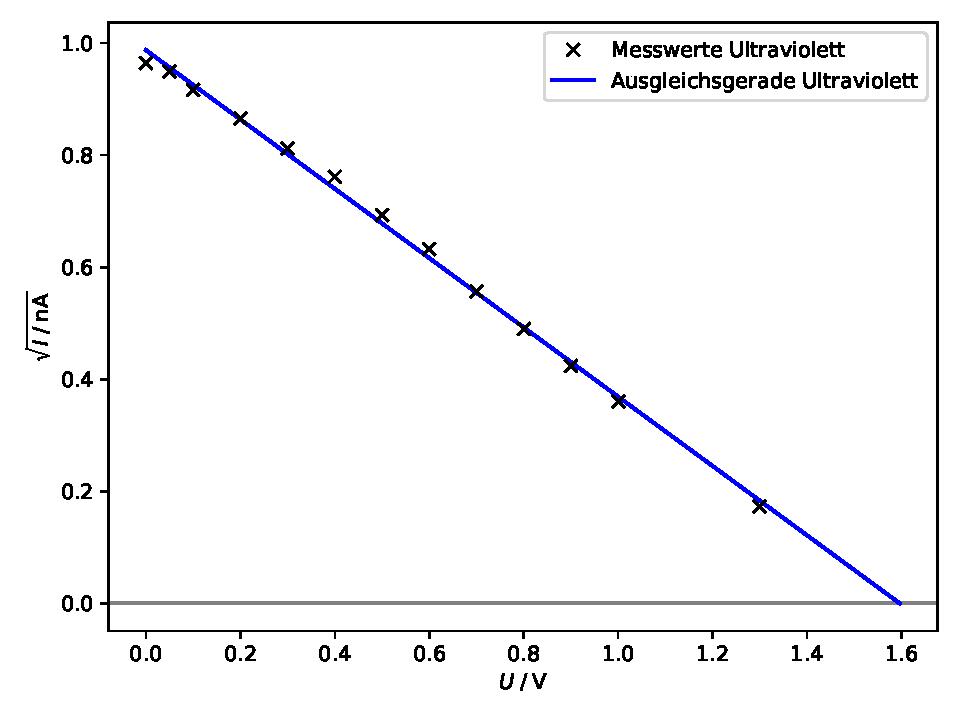
\includegraphics[width=0.8\textwidth]{build/plot_sqrt_ultraviolett.pdf}
    \caption{Die Wurzel des Photostroms und ihre Ausgleichgerade für ultraviolettes Licht, aufgetragen gegen die Spannung.}
    \label{fig:plot_sqrt_ultraviolett}
\end{figure}

\begin{table}
  \centering
  \caption{Fit-Parameter und Grenzspannungen der vermessenen Farben.}
  \label{tab:grenzspannungen}
  \begin{tabular}{c S c c c}
  \toprule
  Farbe &
  $\lambda \mathbin{/} \si{\nano\meter}$ &
  $a \mathbin{/} \si{\nano\ampere\tothe{0.5}\per\volt}$ &
  $b \mathbin{/} \si{\nano\ampere\tothe{0.5}}$ &
  $U_g \mathbin{/} \si{\volt}$ \\
  \midrule
  % \expandableinput{build/table_fitdata.tex}
  Gelb         & 578   & \num{-0.994} ± \num{0.037} & \num{0.432} ± \num{0.010} & \num{0.435} ± \num{0.019} \\
  Grün         & 546   & \num{-1.293} ± \num{0.053} & \num{0.721} ± \num{0.019} & \num{0.558} ± \num{0.027} \\
  Violett      & 435   & \num{-1.025} ± \num{0.013} & \num{1.119} ± \num{0.007} & \num{1.091} ± \num{0.015} \\
  Ultraviolett & 365.5 & \num{-0.618} ± \num{0.010} & \num{0.987} ± \num{0.006} & \num{1.597} ± \num{0.027} \\
  \bottomrule
  \end{tabular}
\end{table}

% \clearpage
\subsection{Bestimmung von \texorpdfstring{$\frac{h}{e}$}{h/e} und der Austrittsarbeit}
\label{sec:auswertung:gelb_full}

Um das Verhältnis aus Planckschem Wirkungsquantum $h$ und Elementarladung $e$
sowie die Austrittsarbeit $A_\text{K}$ zu ermitteln,
können die Grenzspannungen aus \autoref{tab:grenzspannungen}
gegen die jeweilige Lichtfrequenz aufgetragen werden.
Besagtes Verhältnis ist dann die Steigung $a$ der Ausgleichgerade
\[ I = a U_g + b \; . \]
Die Austrittsarbeit lässt sich anhand des y-Achsenabschnitts gemäß $A_\text{K} = - b \cdot e$ bestimmen.

\begin{figure}[H]
  \centering
  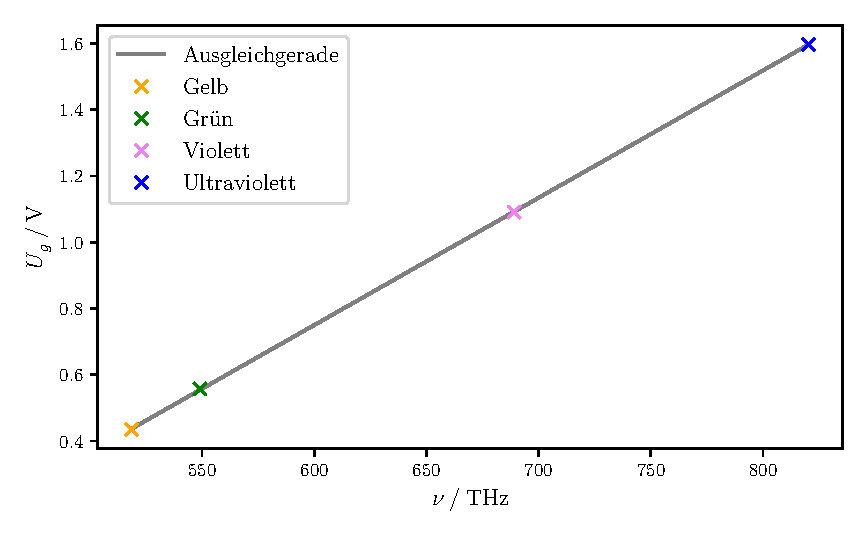
\includegraphics[width=\textwidth]{build/plot_nu_ug.pdf}
  \caption{Grenzspannungen $U_g$ in Abhängigkeit der Lichtfrequenz $\nu$.}
  \label{fig:plot_nu_ug}
\end{figure}

Es ergibt sich
\begin{align*}
  a &= \frac{h}{e} = \SI{3.841(14)e-15}{\volt\second} \\
  b &= \SI{-1.555(9)}{\volt} \\
  A_\text{K} &= \SI{1.555(9)}{\electronvolt} \\
\end{align*}

% \clearpage
\subsection{Nähere Betrachtung des Photostroms gelben Lichts}

Im Folgenden soll näher auf den Kurvenverlauf von \autoref{fig:plot_gelb_full} eingegangen werden.
Insbesondere werden dazu die in der Versuchsanleitung genannten Fragen \cite{versuchsanleitung} beantwortet.

\autoref{fig:plot_gelb_full} zeigt sämtliche \hyperref[tab:werte_gelb]{Messwerte zu gelbem Licht}
und betrachtet die ursprünglichen Werte statt ihrer Wurzel.
Es wurde für Spannungen von $\SI{- 20}{\volt}$ bis $\SI{20}{\volt}$ gemessen,
wobei negative Werte für eine Beschleunigungsspannung
und positive Werte für eine Bremsspannung stehen.

% Für hohe Beschleunigungsspannungen ist zu erahnen,
% dass die Werte auf einen Sättigungswert zulaufen.
% Der lineare Teil von Interesse ist hier im Kontext zu sehen…

\begin{figure}[H]
  \centering
  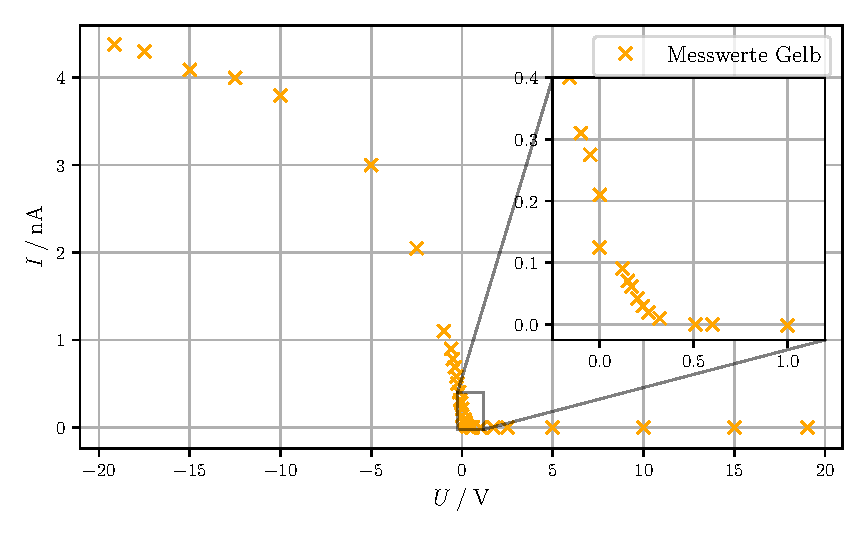
\includegraphics[width=\textwidth]{build/plot_gelb_full.pdf}
  \caption{Photostrom für gelbes Licht, aufgetragen gegen die Spannung.}
  \label{fig:plot_gelb_full}
\end{figure}

\subsubsection*{Warum erreicht die Kurve bei hohen beschleunigenden Spannungen einen Sättigungswert? (Widerspruch zum Ohmschen Gesetz?)}

Aufgrund der endlichen Intensität des auf die Photokathode eintreffenden Lichts
steht nur eine begrenzte Anzahl von Photonen zur Verfügung, um Elektronen auszulösen.
Ist die Beschleunigungsspannung groß genug gewählt,
können alle ausgelösten Elektronen die Anode erreichen.

Das Ohmsche Gesetz postuliert einen proportionalen Zusammenhang von Spannung und Stromstärke: $I = \frac{U}{R}$.
Es gilt jedoch nur für sogenannte Ohmsche Widerstände beziehungsweise in Näherung.
Bei der Photozelle handelt es sich offenbar nicht um einen solchen Ohmschen Widerstand,
da eine Proportionalitätskonstante, d.h. ein Widerstand $R$, nicht ausreicht,
um den Zusammenhang von Spannung und Stromstärke zu beschreiben.
% Das ist anschaulich damit zu begründen,
% dass der Photostrom

\subsubsection*{Durch welche Parameter wird der Sättigungswert festgelegt?
Was trägt dazu bei, dass der Sättigungswert nur asymptotisch erreicht wird?}

Der Sättigungswert ist abhängig von der Lichtintensität,
nicht jedoch von der Wellenlänge.
Letztere sorgt nur für eine schnellere Annäherung an diesen,
da aufgrund der größeren durch die Photonen übertragenen Energie
eine im Schnitt geringere Beschleunigungsspannung zum Erreichen der Anode nötig ist.

Der Sättigungswert wird unter anderem deshalb nur asymptotisch erreicht,
da die Photokathode nicht perfekt evakuiert ist.
Das verbleibende Gas stellt ein Hindernis dar,
welches mit größerer Beschleunigung besser überwunden werden kann.

\subsubsection*{Wie müsste eine Photozelle konstruiert werden,
bei der der Sättigungswert des Photostroms bereits bei endlichen Beschleunigungsspannungen auftritt?}

Wie zuvor beschrieben
sind zwischen Photokathode und Anode befindliche Gaspartikel
für die asymptotische Annäherung an den Sättigungswert zumindest mitverantwortlich.
Um diesen Effekt zu minimieren,
muss die Photozelle daher (besser) evakuiert werden.

\subsubsection*{Warum fällt der Photostrom bei der Gegenspannung $U_g$ nicht abrupt auf $0$ ab,
sondern beginnt bereits für $U > U_g$ zu sinken?}

Wie in \autoref{sec:theorie:fermi_dirac} diskutiert,
haben die Elektronen in der Photokathode aufgrund der Fermi-Dirac-Verteilung unterschiedliche Energien,
sodass auch die zum Lösen dieser benötigte Energie von Elektron zu Elektron variiert.
Daher gibt es Elektronen,
deren Energie trotz $U > U_g$ nicht ausreicht,
um die Anode zu erreichen.

\subsubsection*{Warum kann ein dem Photostrom entgegengerichteter Strom auftreten?}
% (Hinweis: Die Photokathode besteht aus einem Material, das bereits bei $T = \SI{20}{\celsius}$ merklich verdampft.)

% Da das Kathodenmaterial schon bei Zimmertemperatur verdampft \cite{versuchsanleitung},
% provoziert die angelegte Spannung thermische Elektronenemission,
% welche dem Photostrom entgegengerichtet ist.

% siehe rkallo ↓
Da das Kathodenmaterial schon bei Zimmertemperatur ($\SI{20}{\celsius}$) verdampft \cite{versuchsanleitung},
kann sich dieses an der Anode absetzen,
sodass auch dort ein photoelektrischer Effekt auftritt,
welcher dem gewünschten Photoeffekt entgegengerichtet ist
und durch die angelegte Spannung zusätzlich provoziert wird.

\subsubsection*{Warum kann hier bereits bei relativ kleinen Spannungsbeträgen praktisch ein Sättigungswert erreicht werden?}

Dieser ungewünschte Effekt ist klein gegenüber dem eigentlich vorgesehenen Photoeffekt.
% und daher nur für kleine Spannungen und Lichtfrequenzen relevant, wo er…

\subsubsection*{Was kann man über die Austrittsarbeit der Anode sagen, wenn man berücksichtigt,
dass der negative Strom bereits bei der Einstrahlung energiearmen Lichtes ($\lambda \approx \SI{650}{\nano\meter}$) auftritt?}

Die Anode hat eine geringere Austrittsarbeit als die Kathode,
da an dieser unter Einstrahlung energiearmen Lichts offensichtlich mehr Elektronen austreten.
